% exercise sheet with header on every page for math or close subjects
\documentclass[12pt]{article}
\usepackage[utf8]{inputenc} 
\usepackage{latexsym} 
\usepackage{multicol}
\usepackage{fancyhdr}
\usepackage{amsfonts} 
\usepackage{amsmath}
\usepackage{amssymb}
\usepackage{enumerate}
\usepackage{listings}
\usepackage{graphicx}

% Shortcuts for bb, frak and cal letters
\newcommand{\E}{\mathbb{E}}
\newcommand{\V}{\mathbb{V}}
\renewcommand{\P}{\mathbb{P}}
\newcommand{\N}{\mathbb{N}}
\newcommand{\R}{\mathbb{R}}
\newcommand{\C}{\mathbb{C}}
\newcommand{\Z}{\mathbb{Z}}
\newcommand{\Pfrak}{\mathfrak{P}}
\newcommand{\Pfrac}{\mathfrak{P}}
\newcommand{\Bfrac}{\mathfrak{P}}
\newcommand{\Bfrak}{\mathfrak{B}}
\newcommand{\Fcal}{\mathcal{F}}
\newcommand{\Ycal}{\mathcal{Y}}
\newcommand{\Bcal}{\mathcal{B}}
\newcommand{\Acal}{\mathcal{A}}


% Formatierung
\topmargin -2cm 
\textheight 24cm
\textwidth 16.0 cm 
\oddsidemargin -0.1cm

\setlength{\parindent}{0pt}  % !!!!!!! Hier werden leerzeilen erlaubt ohne dass Latex automatisch einrueckt! !!!!!!! %


\graphicspath{ {images/} }


\begin{document}

% Titel
%\title{\textsc{Hacking}\\ \textsc{Abgabe 0}\\{ \normalsize Gruppe X \hfill Daniel Schäfer (2549458)\\ \hfill Anderer}}
%\maketitle  

% alternativer Titel
\noindent
{\Large \textbf{High-level Computer Vision}} \hfill \textbf{06.06.2016}\\
{\Large \textbf{Exercise 4}} 
\raggedleft \hfill Guillermo Reyes (2556018)\\
\hfill Daniel Schaefer (2549458)\\
\hfill Marc Tonsen (2537359)\\
\hfill Dominik Weber (2548553)\\

\pagenumbering{gobble}
\raggedright


\section*{Code Annotations}



\section*{Question 1: Codebook Generation}
\begin{figure}[h]
	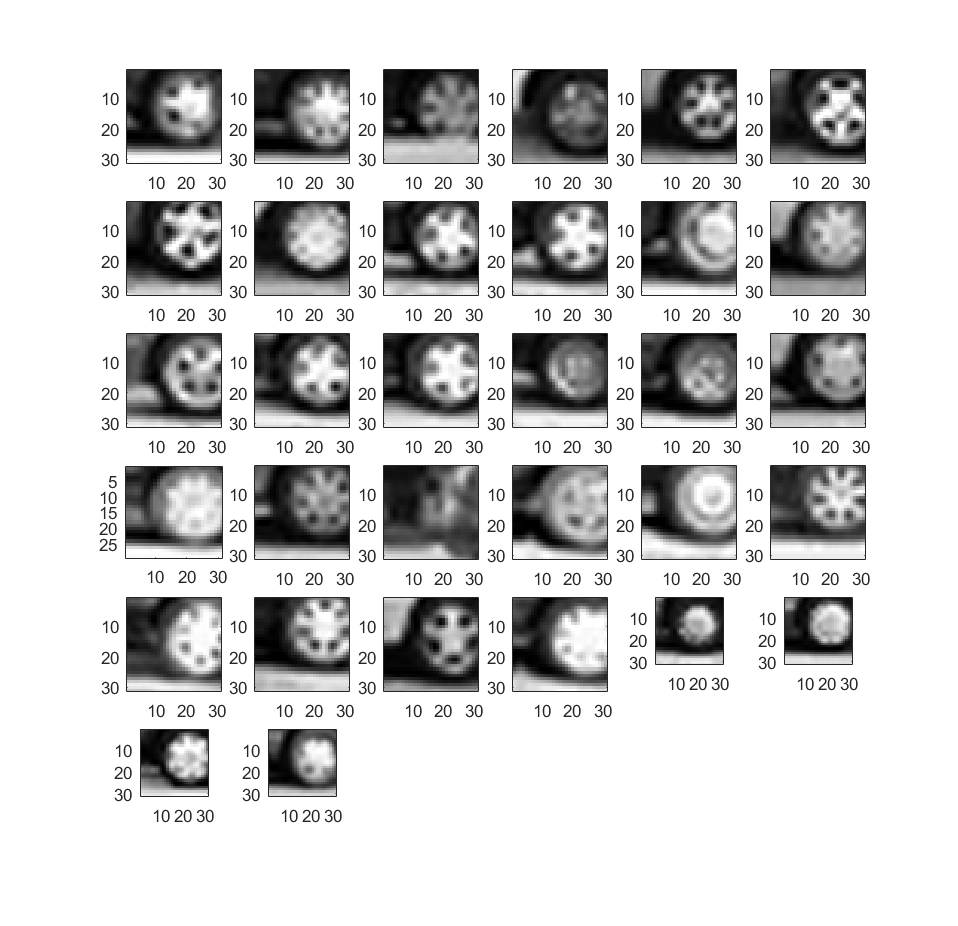
\includegraphics[width=0.5\textwidth]{features1}
	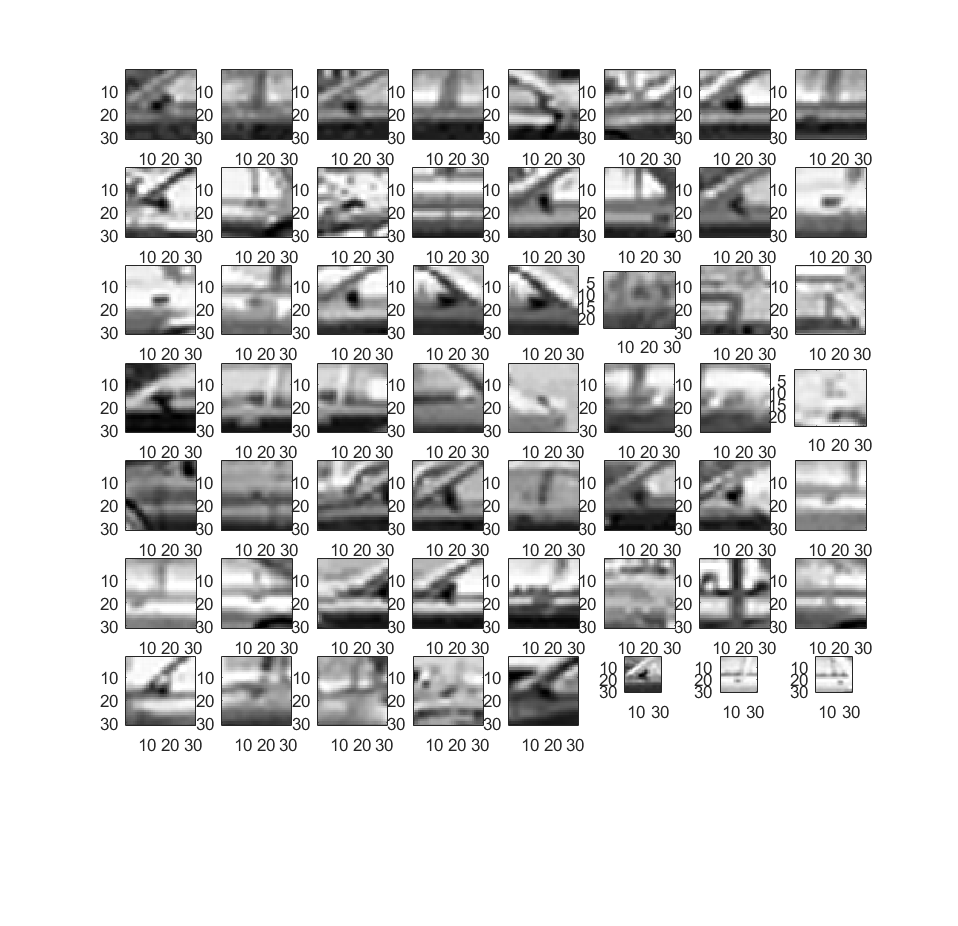
\includegraphics[width=0.5\textwidth]{features2}
	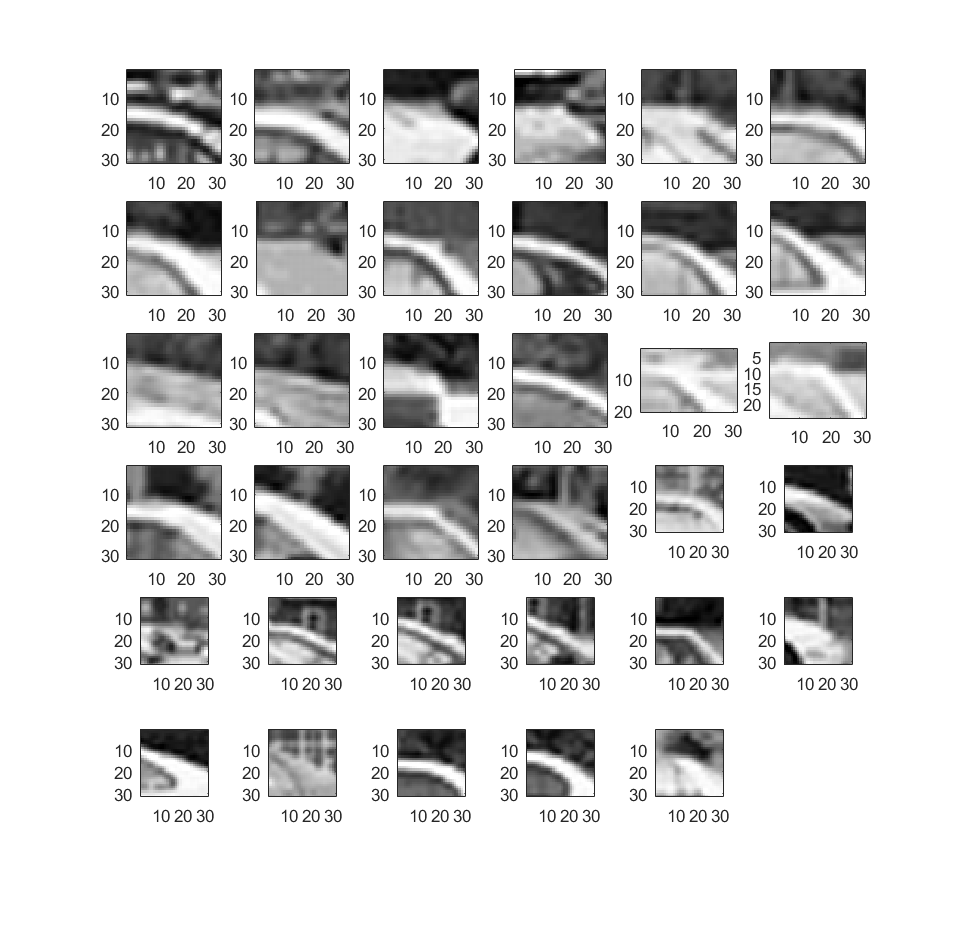
\includegraphics[width=0.5\textwidth]{features3}
	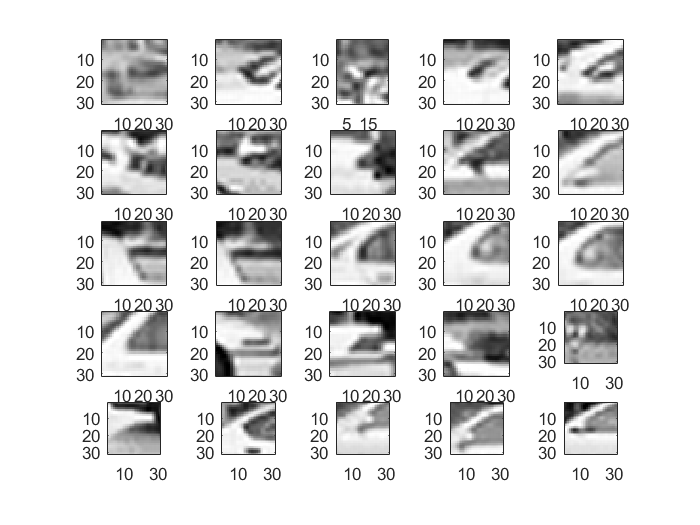
\includegraphics[width=0.5\textwidth]{features4}
		
	\caption{Visualization of several codebook entries. \textit{Upper left}: visualizes the wheels. \textit{Upper right}: the side mirror. \textit{Lower left} curvature in the back part of the roof. \textit{Lower right} appears to be the curvature, mainly in the passenger door window.  }
\end{figure}
As we can see in Figure 1 the learned codebooks make sense from a visual point of view. They seem to capture shapes that are representative for a car. For instance on the upper left we can see the wheels of the car or on the upper right the side mirror. Other images are perhaps not so easily distinguishable, however they represent parts that one would mainly find in a car as opposed to, say, the environment such as the slope in the back part of the roof on the Lower left of Figure 1, or the edge of the passenger window.
\newpage
\section*{Question 3: Occurrence Generation}

\newpage
\section*{Question 4: Recognition}


\end{document}
